\begin{Exercise}[title=Small Networks]
In this exercise we will connect neurons to make simple neural networks. In Neuronify, you can connect a neuron to another neuron just like any other other device, such as those we looked at in the previous exercise. 

\begin{ExePart}
In this part we will make the simplest possible network by connecting one neuron to another. 

Make a small network by doing the following:
\begin{itemize}
\item Create an empty canvas by pressing the menu button in the upper left corner, then press select simulation and click on the empty canvas.

\item Create two neurons, and label them ``A'' and ``B''. You can set neuron labels by pressing a neuron, pressing the gear in the \gearpos  corner. This will open up a tab on the right side of the screen. Press the field marked ``Label:'' and enter the label you want. Complete the operation by pressing Enter. 

\item Connect neuron A to neuron B by clicking on neuron A, grabbing the connection and pulling it to neuron B. 

\item Connect a current clamp to neuron A as in exercise 1. Connect a Voltmeter to both neurons by dragging the voltmeter onto the canvas, pressing it, pressing the gear in the \gearpos corner, and pressing the ``Connect to all neurons''-button.
\end{itemize}

Your canvas should now look like this: \\
\begin{center}
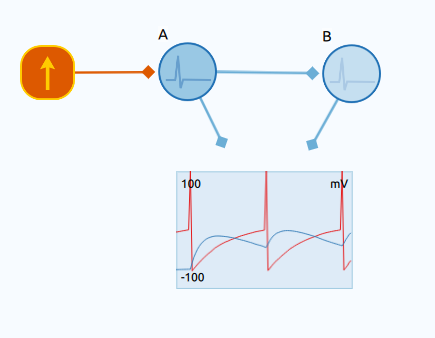
\includegraphics[width=8cm]{two_neurons.png}
\end{center}

Note that the voltage trace from neuron B is very different from neuron A, because neuron A receives a steady current input, while neuron B receives the spikes from A. 

Using the default settings for both neurons, check that 75 mA is the smallest amount of Output Current from the current clamp that still allows neuron B to fire. Now, set the resting potential of both neurons to -70 mV, and attempt to find the minimum current output needed to induce spiking in neuron B.
\end{ExePart}

\begin{ExePart}
In this exercise we will look at a simple convergent connections. Create a new empty canvas. Create two neurons, label them ``A1'' and ``B''. Set the stimulation output of Neuron A1 to 0.5. Connect neuron A1 to neuron B. Create a current generator and connect it to neuron A1. 

We can make add noise to a neuron by adding spike generators. Add to spike generators to the canvas (they are the green squares with question marks on them). Set their rates to 2.0 ms$^{-1}$ and their stimulation output to 0.1. Make one of the generators inhibitory. Connect a voltmeter to both neurons. 

Now your canvas should look like this: 
\begin{center}
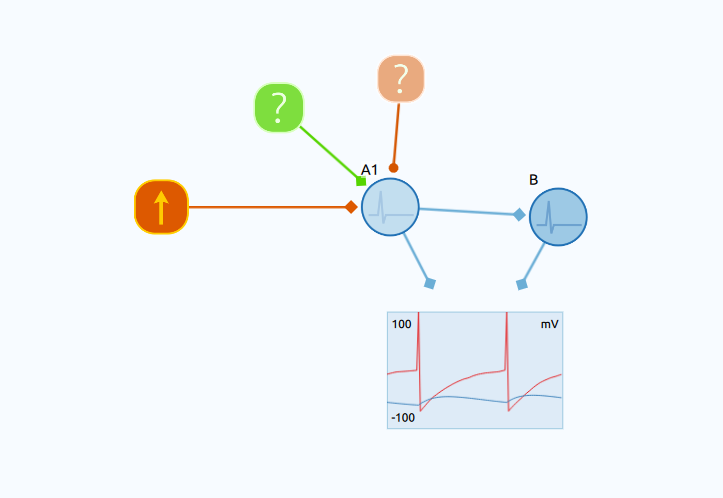
\includegraphics[width=8cm]{two_neurons_noise.png}
\end{center}

Because of the spike generators, there is a chance that neuron B will eventually fire in this circuit, but the odds are astronomically small. Disconnect the spike generators by pressing on the wires going from the generator to the neuron and then pressing the trash can in the lower left corner. 
\begin{itemize}
\item Make several more neurons with Stimulation output 0.5, and connect the current generator to each of them. Label them ``A2'', ``A3'', and so on. How many neurons do you have to connect to neuron B in order to make it fire? 

\item Add excitatory and inhibitory spike generators to each of the neurons A1, A2, \dots. How many neurons do you need to connect to B in order to make it fire now?
\end{itemize}
\end{ExePart}



\end{Exercise}